\documentclass[conference]{IEEEtran}
\IEEEoverridecommandlockouts
% The preceding line is only needed to identify funding in the first footnote. If that is unneeded, please comment it out.
\usepackage{cite}
\usepackage{amsmath,amssymb,amsfonts}
\usepackage{algorithmic}
\usepackage{graphicx}
\usepackage{textcomp}
\usepackage{xcolor}
\usepackage[brazilian]{babel}
\usepackage[utf8]{inputenc}
\usepackage[T1]{fontenc}
\def\BibTeX{{\rm B\kern-.05em{\sc i\kern-.025em b}\kern-.08em
    T\kern-.1667em\lower.7ex\hbox{E}\kern-.125emX}}
\begin{document}

\title{Algoritmo Imunológico Artificial CLONALG}

\author{Bruno Lopes}
\maketitle

\end{abstract}

\section{INTRODUÇÃO}
 O objetivo desse artigo é explorar o Algoritimo Imunológico Artificinal CLONALG para resolver um determinado problema de busca, onde dado um antígeno, devemos gerar uma população de anticorpos para avaliarmos o grau de afinidade com o invazor, para então replicarmos os melhores candidados. A cadeia de sequência do antígeno ira representar um número e a nossa população de anticorpos sera uma matrix aleatória com as nossas soluções candidatas.
\section{Referencial Teórico}
	Os Sistemas Imunológicos Artificiais (SIA) são compostos por modelos inspirados na atividade do Sistema Imunológico Biológico em um organismo. Tais modelos apresentam características adaptativas e evolutivas, sendo possível então a criação de algoritmos imuneinspirados com as mesmas capacidades. Esta técnica constitui uma bioinpiração e faz parte da área da Computação Natural, que surgiu como uma nova área de pesquisa na computação nas ultimas décadas \cite{LNCASTRO}.

    O algoritmo de seleção clonal (CLONALG) é inspirado no princípio de seleção clonal e nos mecanismos de  seleção e  maturação proporcional a afinidade  \cite{LNCASTRO2}. Este algoritmo é  uma abordagem clássica imunológica, cujo princípio básico de funcionamento é classificado como algoritmos evolutivos (AE) e têm se destacado pela eficiente solução de problemas de busca e otimização, principalmente os de caráter combinatório. 
    
    Os  algoritmos evolutivos  propõem um  paradigma de  solução  de problemas  através  da inspiração  na  biologia  evolutiva,  principalmente  na  teoria  da  seleção  natural.  Dada  uma população de indivíduos, os de melhor qualidade têm maior probabilidade de sobrevivência e reprodução,  podendo  continuar  no  processo  de  busca  pela  solução  ótima.  Esta  é  uma característica  da  evolução  das  espécies  que  também é  observada  em alguns  algoritmos  de sistemas imunológicos artificiais, como o algoritmo CLONALG, que são baseados na teoria da seleção clonal e maturação de afinidade \cite{LNCASTRO2}.
    
    Na sequência apresenta-se o algoritmo CLONALG \cite{SS}
    \begin{itemize}
    
    \item Passo 1: Gere uma população (P) com N anticorpos (soluções candidatas);
    
    \item Passo  2:  Avalie  a  afinidade  (função  objetivo)  de  cada  anticorpo  e  selecione  (processo de seleção) os n melhores anticorpos da população P, obtendo o conjunto Pn; 
    
    \item Passo 3: Reproduza  (processo de clonagem) os  n melhores anticorpos selecionados, gerando uma  população  (C)  com  Nc  clones; 
    \item Passo 4: Submeta a população de clones (C) a um processo de hipermutação; 
    
    \item Passo 5: Avalie a afinidade de cada anticorpo pertencente a (C*) e re-selecione os n melhores anticorpos  (C*{n})  e os  adicione a  população P  descartando  os anticorpos  de pior qualidade; 
    
    \item Passo 6: Substitua d anticorpos de baixa afinidade por novos anticorpos (P{d}) (diversidade ou metadinâmica). Os anticorpos com baixa afinidade possuem maior probabilidade de serem substituídos. Os novos anticorpos sáo gerados da mesma forma que os; 
    \item Passo 7: Repita os passos de 2 a 6 até satisfazer o critério de parada. 
    \end{itemize}
    
\section{Metodologia Experimental}
    

    Com base no pseudo código apresentado em \cite{LNCASTRO2} conseguimos replicar a solução. A Figura 1 foi utilizada como antigeno alvo para a funcão objetivo, que selecionada os melhores anticorpos, gerando assim uma nova populacão de possiveis candidados.
 
    O número medio de iterações necessárias para encontrar nossa solução foi satisfatorio, com apenas 73.9 gerações conseguimos satisfazer nossa condição de parada. 
 	\begin{figure}[htbp]
    \begin{center}

    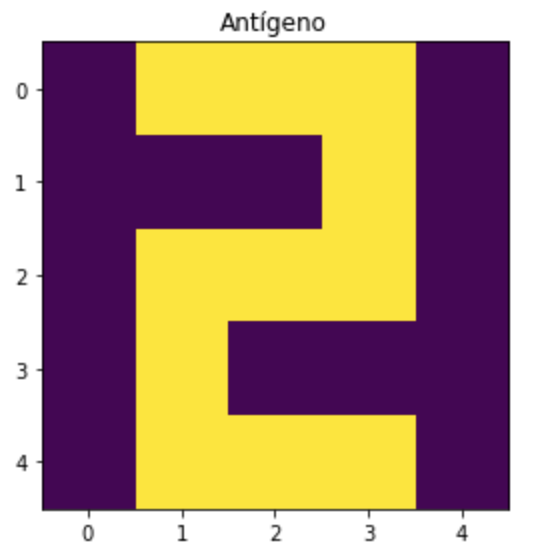
\includegraphics[scale=0.5]{antigeno.png}
    \caption{Imagem que descreve antígeno a ser entrado} \label{gdimotes}
    \end{center}
    \end{figure}

    Foram realizados varios testes alterando o tamanho da população e a taxa de mutação. O resultados apresentado na Tabela 1, foram gerados rodando a aplicação 10 vezes para cada configuração. Estamos exibindo um valor médio de todas as iterações realizadas na fase de testes e com isso conseguimos tirar algumas conclusões.
    
    \begin {table}
    \caption {Resumo experimentos}
    \begin{center}
      \begin{tabular}{ l | c | r }
        \hline
        População Anticorpos&	\% mutação&	média gerações&	\\ \hline
        25&	1.00\%&		961.46&	 \hline
        25&	2.00\%&		848.12& \hline
        25&	10.00\%&	592.55& \hline
        16&	1.00\%&		270.90&	  \hline
        16&	2.00\%&		147.33& \hline
        16&	10.00\%&	73.9&	 
        \hline
      \end{tabular}
      \end{center}
    \end{table}
 
    É possível perceber que exite um comportamento diferente em cada configuração. Ao reconfigurarmos alguns parametros, são necessarios algumas iterações a mais para se chegar a uma solução. 
    
    Com uma taxa de mutação muito baixa, não temos muita variação na população de anticorpos, consequentemente a precisamos esperar um tempo maior convergir. Isso fica claro quando olhamos os resultamos aprsentados na Tabela 1.
    
 
\section{Resultado e Discussão}

   O Algoritmo Imunológico Artificial CLONALG encontra boas soluções não precisando de um alto número de iterações para se chegar a solução objectivo. 
   
   Como mostra em \cite{SS}, podemos ver o ganho de performance comparando os resultados do CLONALLG com Algoritmo Genético. O Algoritmo Imunologico foi capaz de obter soluções de melhor qualidade para maioria das instancias \cite{SS}.
   
   Isso se deve a solução proposta de clonagem dos melhores individuos, fazendo assim com que os de maior afinidade continuem na população, descatando assim anticorpos de pior qualidade.
   
\section*{Conclusão}


\begin{thebibliography}{00}

\bibitem{LNCASTRO} L.  N.  de  Castro.  “Engenharia  Imunológica:  Desenvolvimento  e  Aplicação  de  Ferramentas Computacionais  Inspiradas  em  Sistemas  Imunológicos  Artificiais”.  Tese  de  Doutorado,  Faculdade  de Engenharia Elétrica e de Computação, Universidade Estadual de Campinas, Campinas, Brasil, 2001.

\bibitem{LNCASTRO2} L. N. de Castro and J. F. Von Zuben.  The clonal selection algorithm with engineering applications. In: Workshop Proceedings of Gecco, Workshop on Artificial Immune Systems and Their Applications, 2000, Las Vegas. p. 36-39, (2000)

\bibitem{SOUZA} Souza, Simone & Romero, Ruben. (2014). Algoritmo Imunológico Artificial CLONALG e Algoritmo Genético Aplicados ao Problema do Caixeiro Viajante. 10.5540/03.2014.002.01.0106. 

\bibitem{LNCASTRO3} L. N. de Castro and J. I. Timmis. Artificial immune systems: A new computational intelligence approach, Springer-Verlag, Heidelberg. 2002.

\bibitem{SS} S. S. F. Souza and R. Romero, “Algoritmo Imunológico Artificial CLONALG e Algoritmo Genético Aplicados ao Problema do Caixeiro Viajante,” vol. 2, pp. 1–6, 2014.
\end{thebibliography}

\end{document}
